% !TEX root = ../thesis.tex
\section{Analýza akustického signálu a jeho parametrizace}
\label{chap:construction:analysis}

Rozpoznávání řeči se věnuje nemalé usílí již od 50. let 2O. století a v současné době nikoho nepřekvapí téměř bezchybně fungující obecný rozpoznávač v mobilních zařízeních. Pro obecné systémy dokonce existují korpusy s desítkami či stovkami a více hodin promluv, které je možné využít při vytváření těchto systémů.

Tyto korpusy však obsahují ve většině případů pouze \uv{standardní}\footnote{Slovením spojením \uv{standardní řeč} je myšlena řeč neobsahující vyrazné řečové vady, případně jiné formy produkce a často v nepřílíš akusticky náročném prostředí.} řeč. Pokud je snaha vytvořit nebo ověřit funkčnost systému za specifických podmínek (ať už se jedná o rušné prostředí či speciální typy promluv), tak je nezbytné získat potřebná data.

\subsection{Analýza získaných dat}
\label{chap:construction:analysis:data}

Po dokončení anotace obsahuje korpus přes 10 hodin akustických záznamů promluv a více či méně přesných přepisů\footnote{I přes nemalou snahu a několikastupňovou kontrolu, je téměř jisté, že by nebylo obtížné najít přepis, který obsahuje chybu například ve formě překlepu.}. Když jsou k dispozici data je možné se podívat na specifika EL řeči a případně porovnat se zdravým řečníkem.

Pro potřeby porovnání byl použit začátek promluvy \textit{\uv{Akcie Komerční banky...}}. Tuta promluva je součástí standardní množiny vět používaných při vytváření řečových korpusů na KKY při ZČU. Tím pádem je k dispozici v relativně velkém množství příkladů pro zdravé řečníky a také je součástí korpusu EL řeči.

Na obr. \ref{fig:construction:el_speech} a \ref{fig:construction:normal_speech} je zobrazen průběh signálu a spektrogram vybrané promluvy. Už na první pohled je možné zaznamenat určité rozdíly. Prvním takovým je délka promluvy, v případě zdravého řečníka je o celou 1 vteřinu kratší než v případě EL řeči. Tempo řeči je samozřejmě velmi individuální, ale z principu je EL řeč pomalejší. Z průbehu signálu na obr. \ref{fig:construction:el_speech} je patrné, že řečník dělá výraznější pauzy mezi jednotlivými slovy promluvy. To může být způsobené například potřebou naplnit jícen vzduchem. Po TL je dýchání realizováno přes tracheu a pokud nebyl voperován shunt (více v \ref{chap:cause:treatment:tracheo}), tak je trvale oddělen hrtan a hltan. Přesto, pro produkci některých neznělých fonémů je potřeba exhalovat vzduch z dutiny ústní. Zkušený EL řečník to dělá naprosto automaticky, nicméně \uv{polykání} vzduchu zabere nějaký čas. Nevyhnutelným důsledkem je pak velmi častý výskyt samovolného říhání v průběhu promluvy\footnote{Fakt, že je říhání jako neřečová událost běžnou součástí téměř každé promluvy, vedl k ignorování těchto událostí během anotace.}.

\begin{figure}[hbpt]
  \centering
  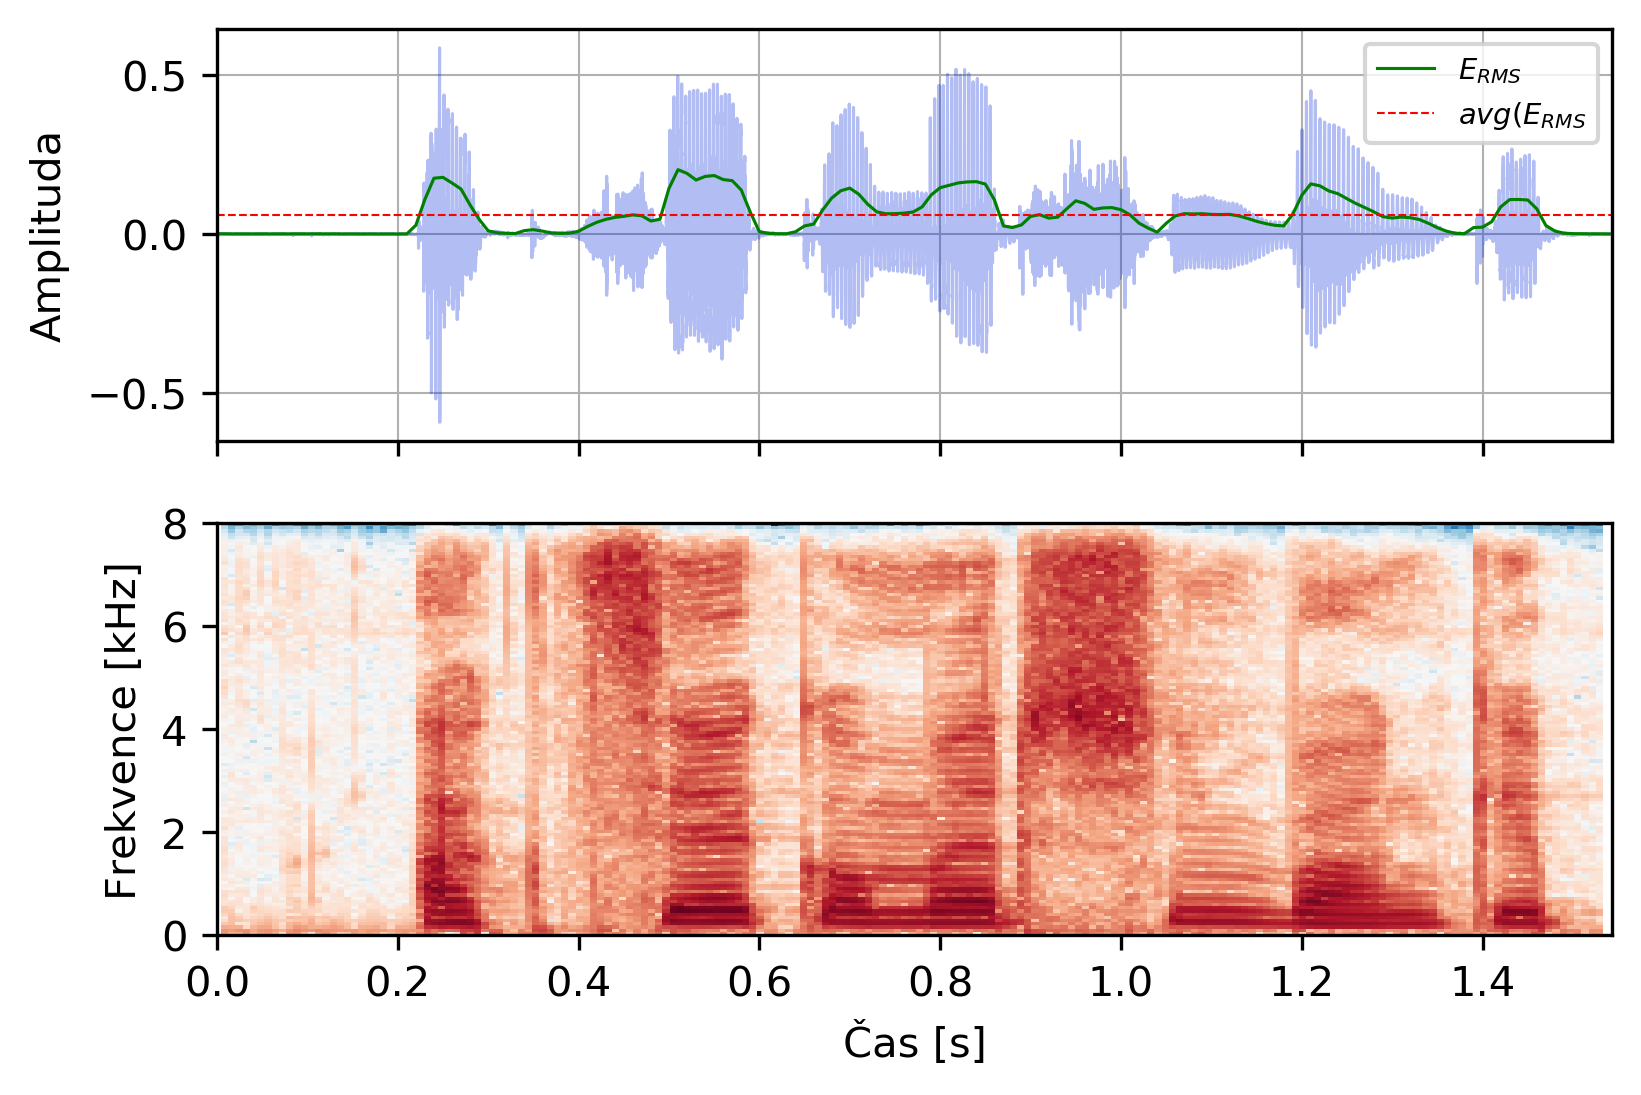
\includegraphics[width=0.9\textwidth]{./ch5-construction/img/energy_spec_normal.png}
  \caption{Průběh a spektrogram promluvy a vyznačenou energií promluvy.}
  \label{fig:construction:normal_speech}
\end{figure}

Dalším důvodem může být je nutnost správné artikulace. Při používání EL je to nezbytné, aby bylo produkované řeči alespoň trochu dobře rozumnět. A pokud se dobře artikuluje, tak není snadné mluvit rychle. Při nahrávání bylo také velmmi běžné, že v průběhu promluvy řečník udělal pauzu, aby mohl lépe umístit EL, protože jeho umístění má velký vliv na kvalitu produkované řeči. Nicméně je třeba říci, že tempo není a priory pro ASR systémy problém, protože různá délka fonémů je v relativně snadno modelována, např. v \textit{HMM} přechodem ze stavu do stejného stavu.

Dalším způsobem jak ukázat rozdíly mezi promluvou zdravého řečníka a řečníka s EL je srovnání ve frekvenční oblasti. Pro větší názornost jsou na obr. \ref{fig:construction:spectrogram} vedle sebe zobrazeno spektrum ukázková promluva zdravého řečníka (\ref{fig:construction:spectrogram:normal}) a toho s EL (\ref{fig:construction:spectrogram:el}). Obsah obou promluv je identický a přesto jsou obě spektra odlišná.

Prvním markantním rozdílem je mnohem větší zastoupení šumu v úsecích \uv{ticha} na obr. \ref{fig:construction:spectrogram:el}. To je nepochyně způsobnemo samotným EL, který řečník nevypíná mezi jednotlivými slovy. Na obr. \ref{fig:construction:el_speech} je to také zřetelně patrný, zejména na průběhu energie, šum zejména před prvním a druhým slovem promluvy. Zajímavá je přítomnost šumu v célém frekvenčním spektru, přestože EL produkuje konstantní buzení. Toto buzení je ve spektru, na obr. \ref{fig:construction:spectrogram:el}, viditelná jako výrazná souvislá linie v nízkých frekvencích. Přitomnost šumu ve vyšších frekvencích je způsobena umístěním mikrofonu, který je nalepen na pokožku a tím pádem snímá namodulované vibrace, přenášené měkkou tkání. Tento fakt se potvrdil v dalších etapách nahrávání (viz část \ref{chap:construction:normalization:corpus}), kde je použit studiový mikrofon vzdálený od úst minimálně 15 cm a tyto vibrace již nezaznamenává. Nicméně z pohledu použitelnosti nějakého budoucího systému je nezbytné počítat i se situací, kdy mikrofon bude zaznamenávat i vibrace přenášené tkání.

Dalším markantním rozdílem je absence vyšších frekvencí u většiny produkovaných fonémů. Vyjímku tvoří afrikáty $/c/$ a $/\check{c}/$, u kterých jsou hlasivky (u zdravého jedince) v klidu a vznikají uvolněním nahromaděného vzduchu v dutině ústní\footnote{Nahromadění vzduchu je realizováno přitisknutím jazyka k přední/zadní části horního patra.} \cite{Psutka2006}. V tomto případě není, u řečníka po TL, principiálně tento mechanizmus produkce těchto fonému ovlivněn. Problémem teoreticky může být zdroj vzduchu, jelikož jej z plic není možné dostat do dutiny ústní, ale jak už bylo zmíněno (a spektrogram to potvrzuje) zkušený uživatel EL se dokáže adaptovat.

Absence vyšších frekcencí se dá vysvětlit použitím EL, kde samotný EL má vždy konstantní frekvenci buzení a dále tím, že nedochází k modulaci v ve všech dutinách vokálního traktu. Nicméně nejdůležitější složky, zajišťující srozumitelnost, se vyskytují ve frekvenčním pásmu od 1 kHz do 3 kHz. Vyšší frekvence se a priory podílejí na zabarvení hlasu.

\begin{figure}[htpb]
  \centering
  \begin{subfigure}[b]{0.4\textwidth}
    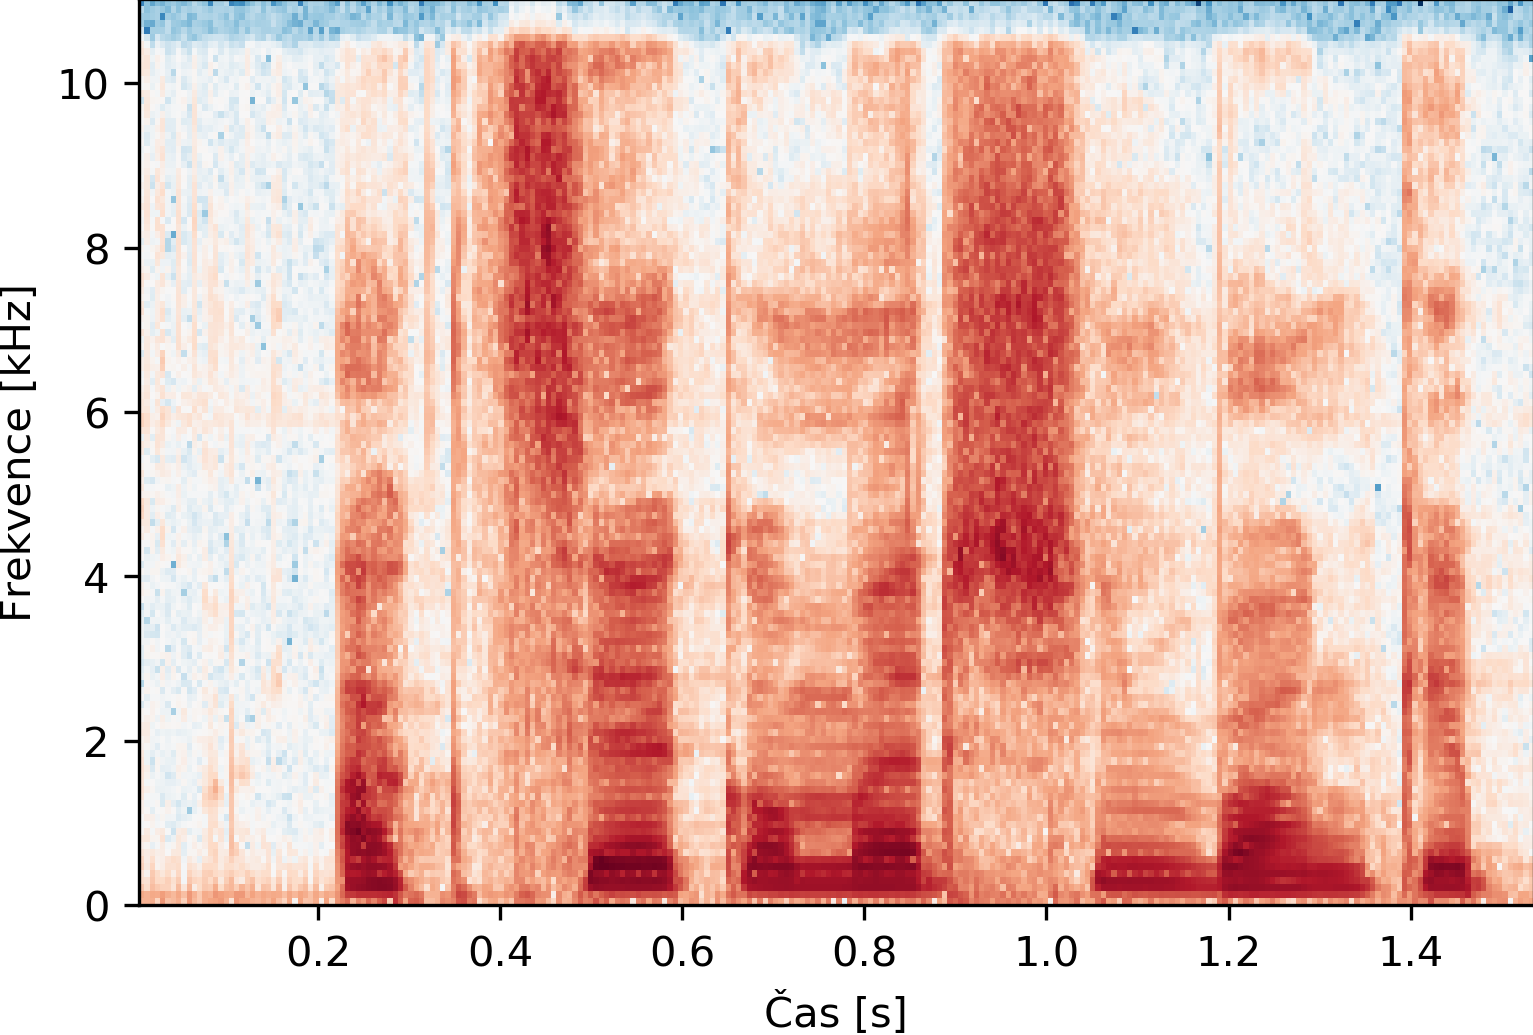
\includegraphics[width=\textwidth]{./ch5-construction/img/spectrogram_normal.png}
    \caption{Zdravý řečník}
    \label{fig:construction:spectrogram:normal}
  \end{subfigure}
  %
  \begin{subfigure}[b]{0.4\textwidth}
    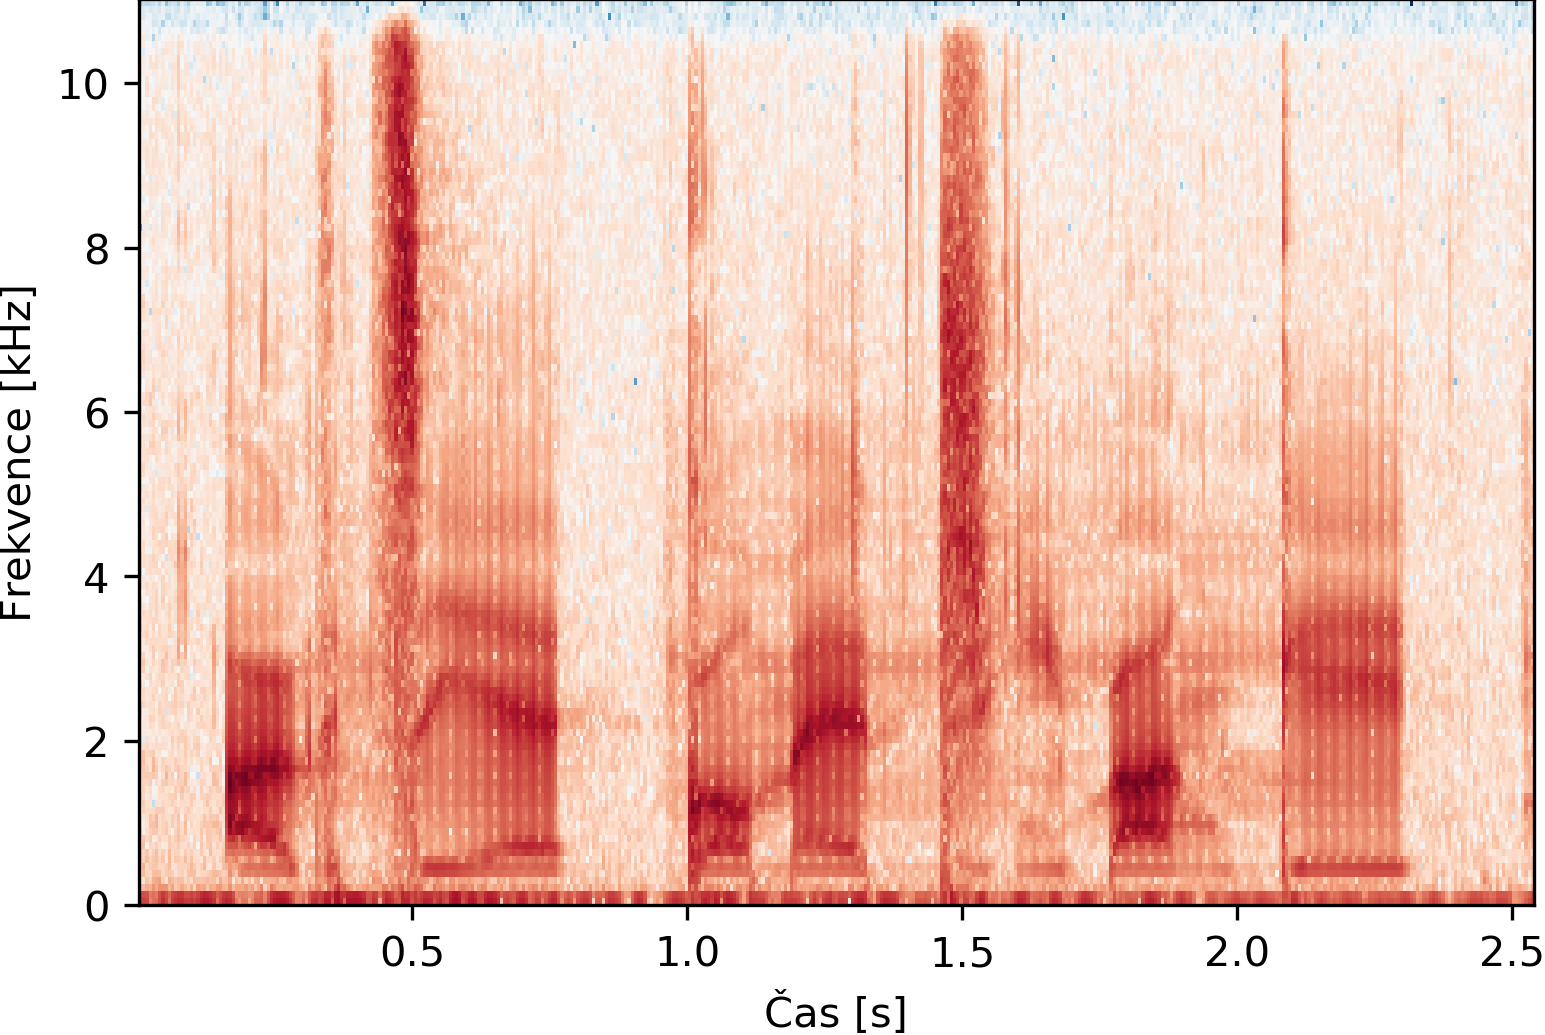
\includegraphics[width=\textwidth]{./ch5-construction/img/spectrogram_el.png}
    \caption{EL řečník}
    \label{fig:construction:spectrogram:el}
  \end{subfigure}
  \caption{Spektrogram promluvy \uv{Akcie Komerční banky} dvou řečníků.}
  \label{fig:construction:spectrogram}
\end{figure}

Dalším způsobem jak porovnat řeč zdravého řečníka a tím s EL je pomocí analýzy jednotlivých fonémů. Na obr. \ref{fig:construction:phonemes} jsou zobrazeny průběhy amplitudy v čase\footnote{Hodnoty času, na obr. \ref{fig:construction:phonemes}, odpovídají časům výskytu v původní promluvě.} pro fonémy $/k/$, $/m/$ a $/\check{c}/$. V případě $/k/$ a $/m/$ (1. a 2. průběh) se jedná o okluzivy, kde v prvním případě se jedná o neznělou plozivu a druhém o znělou plozivu. Tyto fonémy obecně vznikají uzavřením vydechovaného proudu vzduchu, pomocí artikulačních orgánů, což se projeví jako krátká pauza (tzv. okluze). Po té následuje náhlé jednorázové překážky a únik nahromaděného vzduchu, tzv. exploze \cite{Psutka2006}. Takto popsáno to samozřejmě funguje u zdravého jedince, ale u EL řečníka jde principiálně o stejný mechanizmus. S tím rozdílem, že vzduch nepochází z plic, ale z hltanu. Dalším rozdílem je samozřejmě absence hlasivek.

\begin{figure}[htpb]
  \centering
  \begin{subfigure}[b]{0.42\textwidth}
    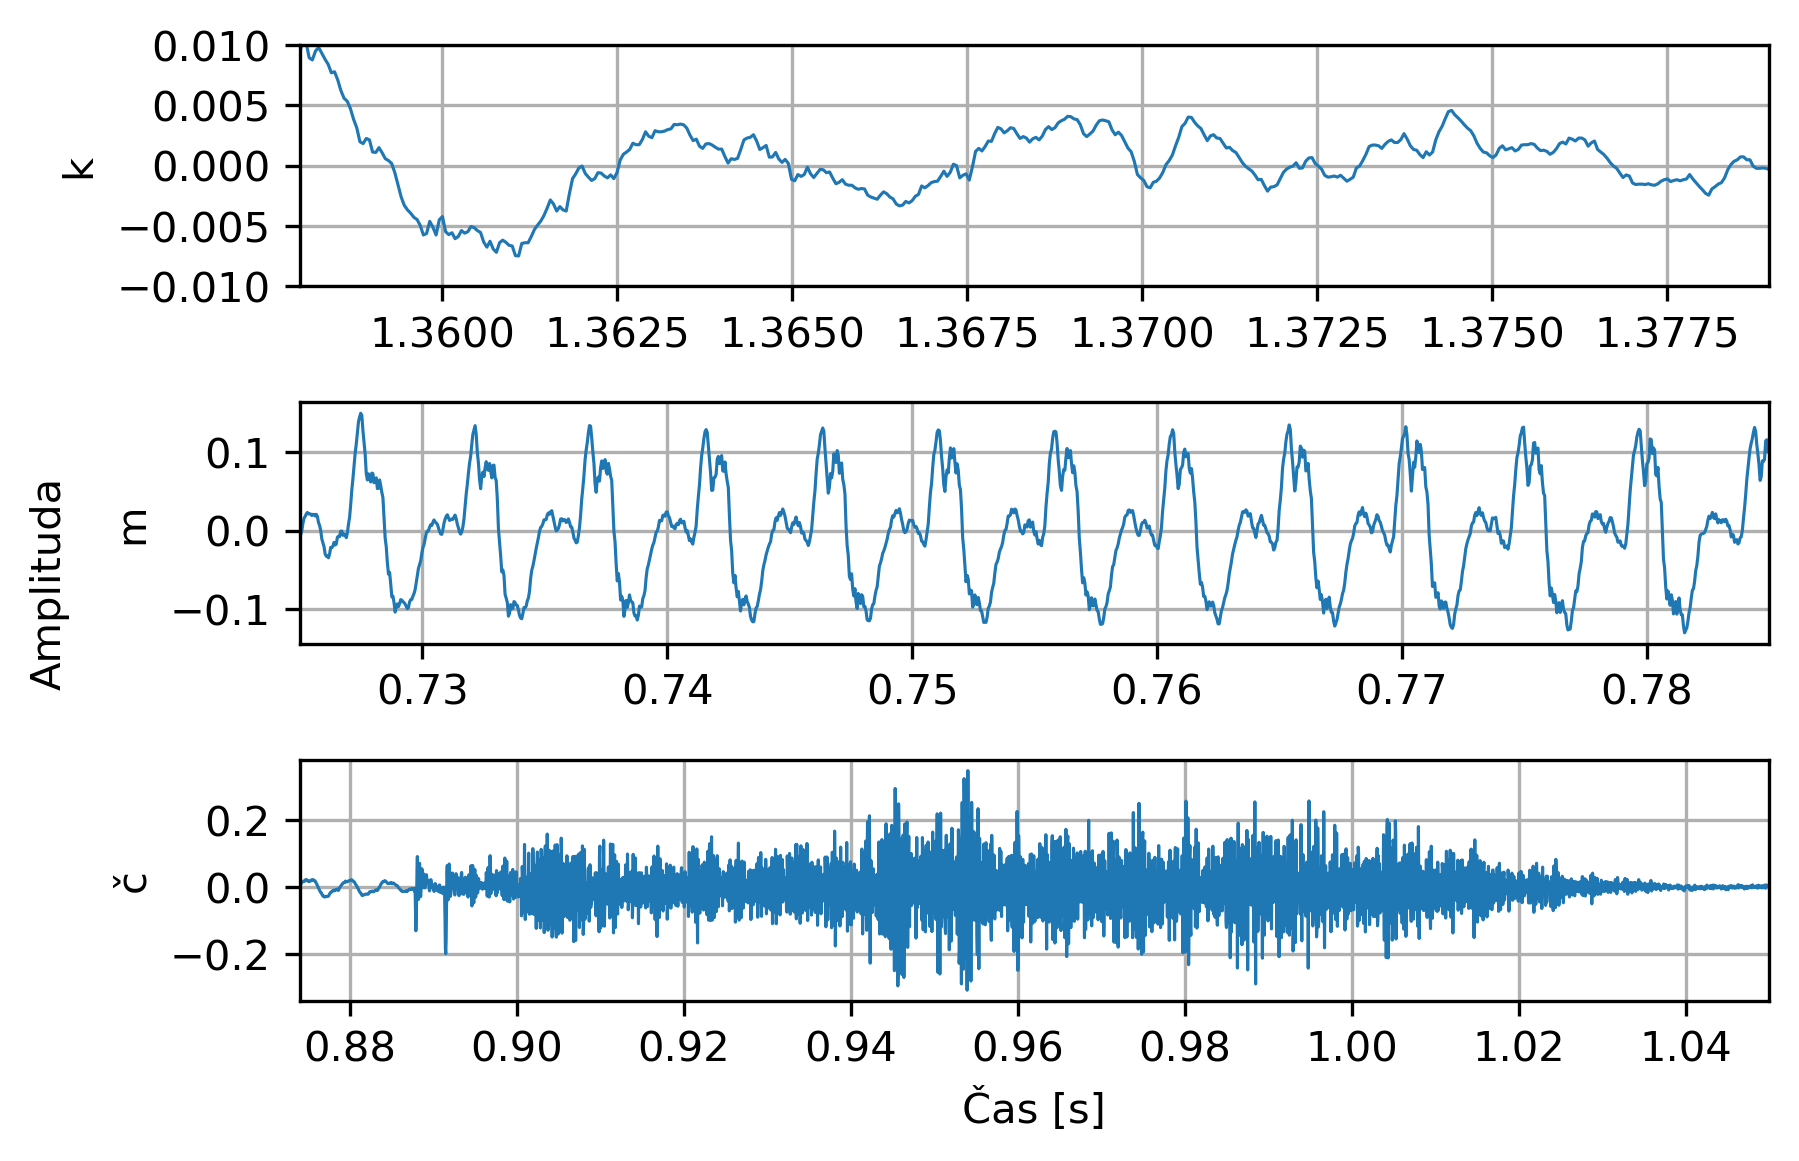
\includegraphics[width=\textwidth]{./ch5-construction/img/phonemes_normal.png}
    \caption{Zdravý řečník}
    \label{fig:construction:phonemes:normal}
  \end{subfigure}
  %
  \begin{subfigure}[b]{0.42\textwidth}
    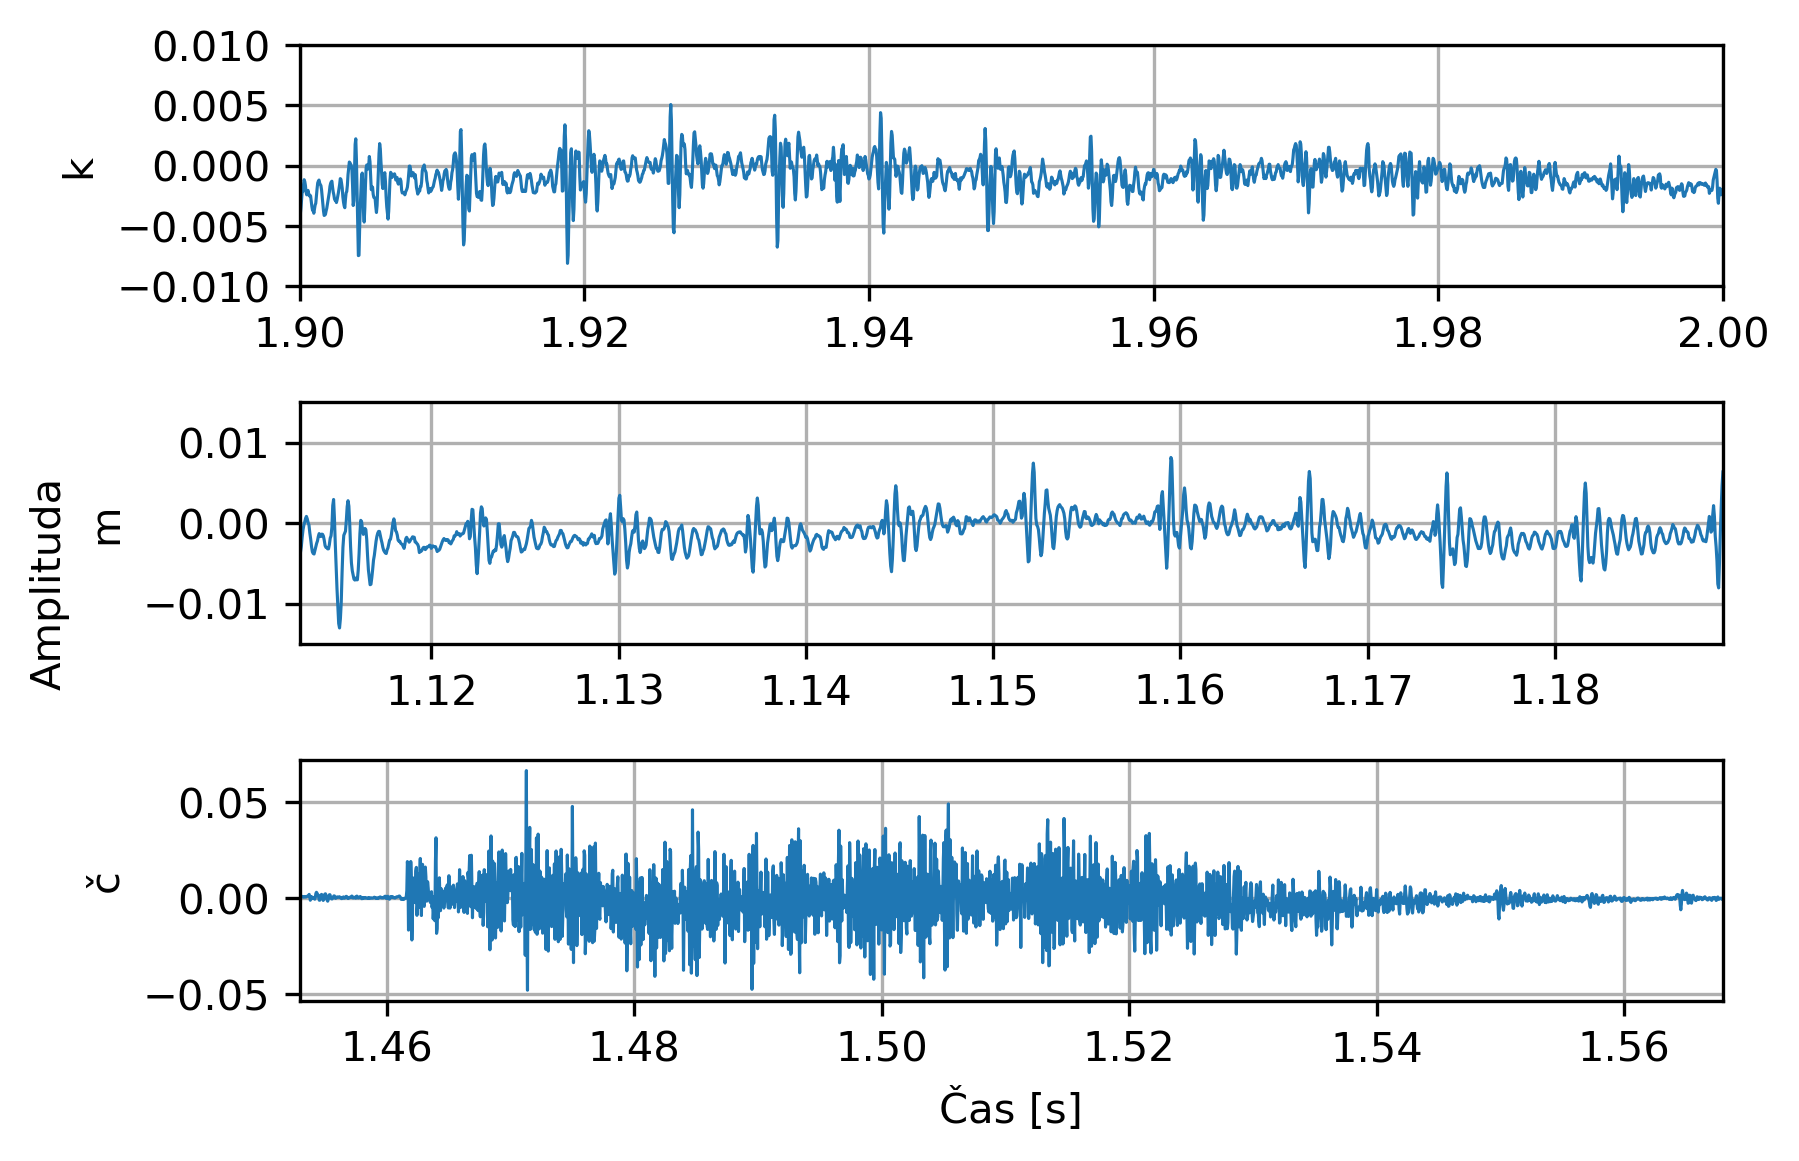
\includegraphics[width=\textwidth]{./ch5-construction/img/phonemes_el.png}
    \caption{EL řečník}
    \label{fig:construction:phonemes:el}
  \end{subfigure}
  \caption{Ukázky průběhů amplitudy pro fonémy $/k/$, $/m/$ a $/\check{c}/$.}
  \label{fig:construction:phonemes}
\end{figure}

Foném $/k/$ představuje zástupce neznělých fonémů, ty se vyznačují tím, že do jejich produkce nezasahují hlasivky, které jsou v klidu. Zdrojem buzení je tedy šum. Pokud se podíváme na průběh amplitudy v čase u zdravého řečníka (obr. \ref{fig:construction:phonemes:normal}), tak zde není vidět žádný periodický signál. Hlasivky jsou tedy opravdu v klidu. Oproti tomu u EL řečníka (obr. \ref{fig:construction:phonemes:el}) je jasně patrné, že je zde přítomno aktivní buzení vytvořené EL. Na obr. \ref{fig:construction:freq:k} je pak zobrazeno tzv. amplitudové spektrum, které znázorňuje vývoj amplitudy signálu ve frekcenci pro oba řečníky. V případě zdravého řečníka odpovídá vývoj očekávání tedy, že zde není žádná výrazná frekvence a také, že nedochází k výraznému útlumu. Přestože se v obou případech jedná o stejný foném, tak z časového i frekvešního průběhu amplitudy je zřejmé, že parametry signálu se u obou řečníku diametrálně liší.

\begin{figure}[hbpt]
  \centering
  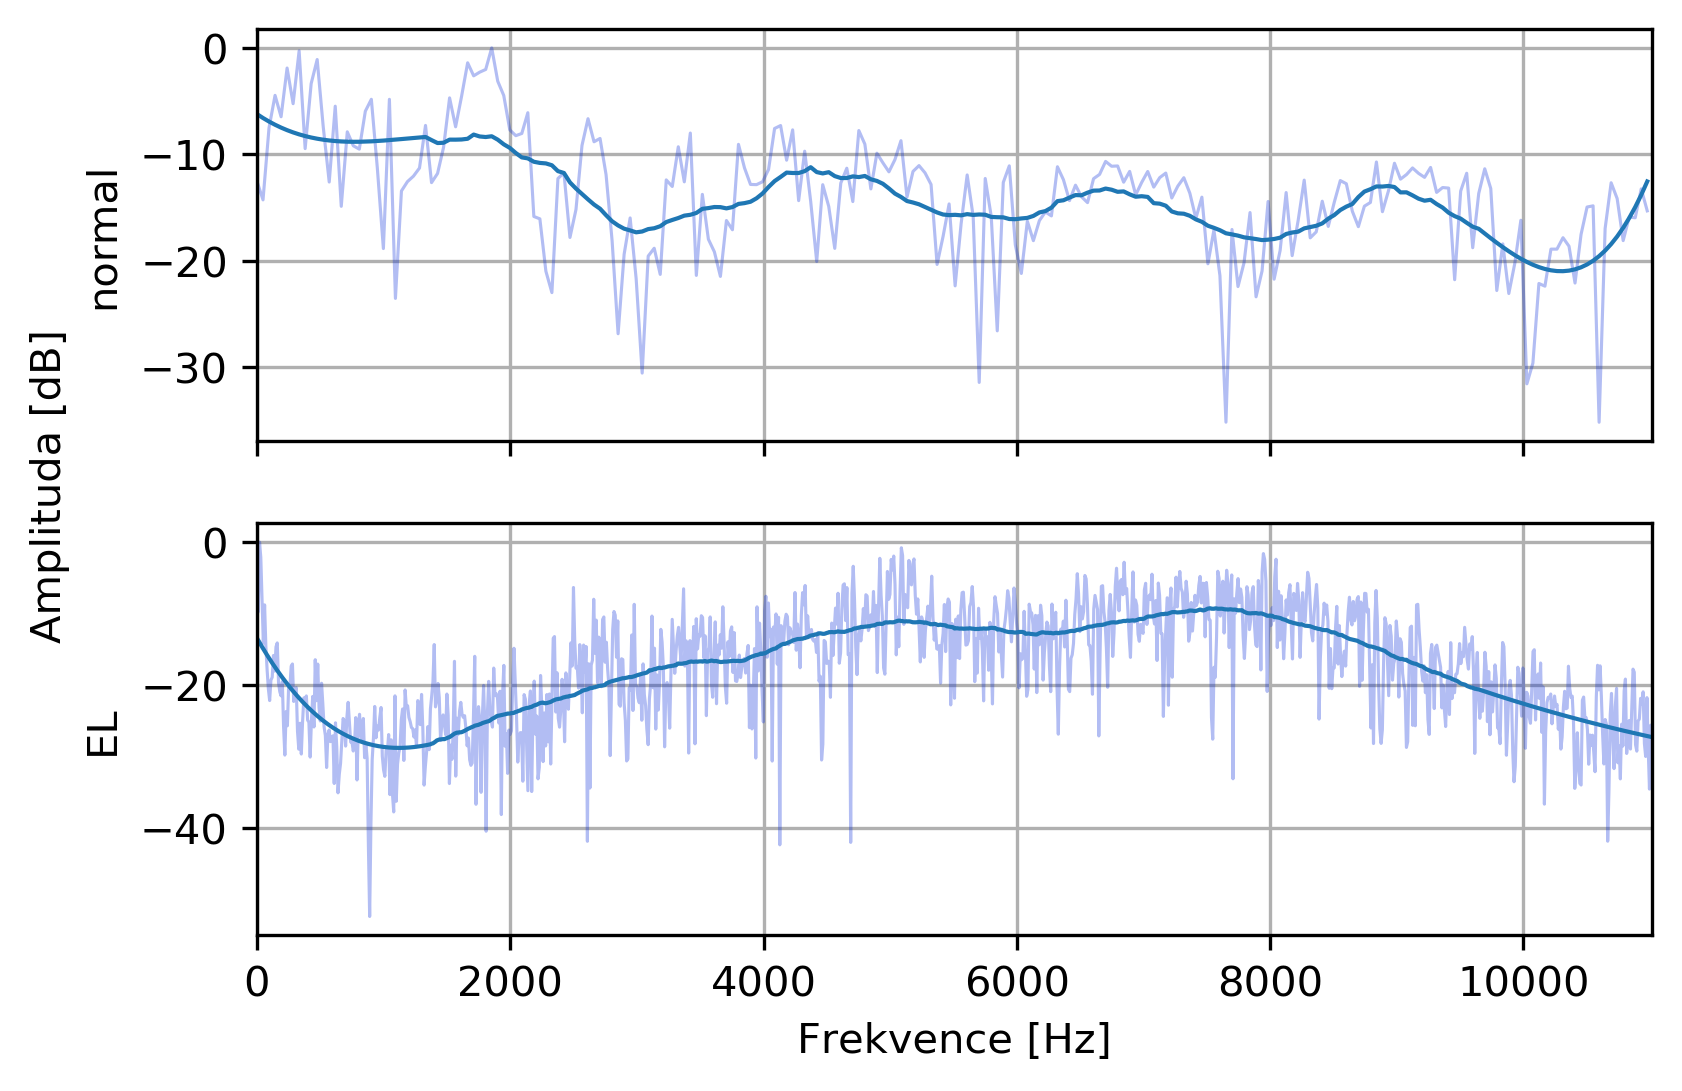
\includegraphics[width=0.9\textwidth]{./ch5-construction/img/freq_analysis_(k).png}
  \caption{Vývoj amplitudy fonému $/k/$ ve frekvenci zdravého (horní) a EL (dolní) řečníka.}
  \label{fig:construction:freq:k}
\end{figure}

Jako druhý ukázkový foném slouží $/m/$. Opět se jedná o plozivu, ale v tomto případě o znělou. U těchto fonémů hrají velký vliv hlasivky, protože jsou zdrojem buzení. Z obr. \ref{fig:construction:phonemes:normal} je krásně zřetelné buzení ve formě perodického průběhu amplitudy. Narozdíl tomu, u EL řečníka (obr. \ref{fig:construction:phonemes:el}) je také vidět periodický signál, ale úplně jiného průběhu. Svým způsoběm dost podobný tomu, který je zřetelný u fonému $/k/$. Rozdíl je zřetelný i ve frekvenční oblasti (obr. \ref{fig:construction:freq:m}), kdy u EL řečnía nedochází útlumu ve střední oblasti frekvenčního spektra.

\begin{figure}[hbpt]
  \centering
  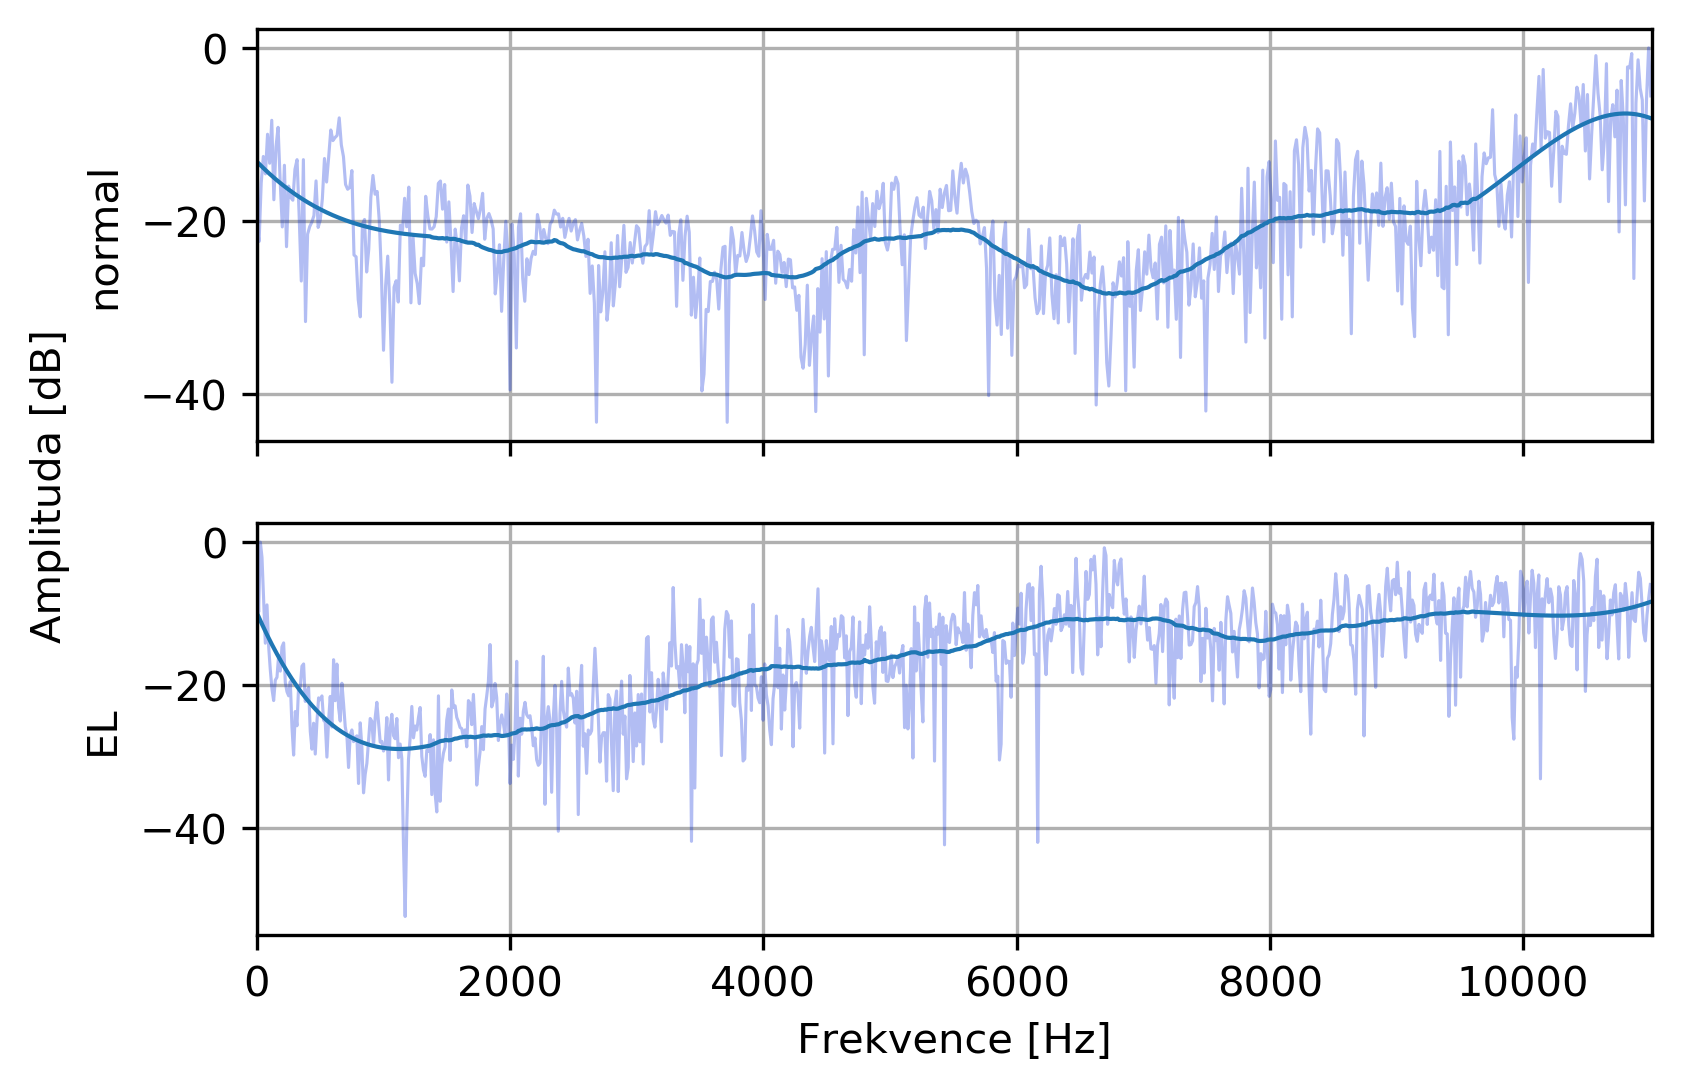
\includegraphics[width=0.9\textwidth]{./ch5-construction/img/freq_analysis_(m).png}
  \caption{Vývoj amplitudy fonému $/m/$ ve frekvenci zdravého (horní) a EL (dolní) řečníka.}
  \label{fig:construction:freq:m}
\end{figure}

Posledním úkázkovým fonémem je již zmiňované $/\check{c}/$. Jedná se o neznělý foném, který vzniká přiložením jazyku k zadní části horního patra. Tím je zadržen vzduch v dutině ústní a vzniká krátká pauza. Uvolněním pak dochází k explozi a vytvoření zvuku. Do produkce se nezapojují hlasivky a produkovaný zvuk by měl být dostatečně intenzivní, aby jej (v případě EL řečníka) tolik neovlivňoval EL. Tím pádem by měl být průběh signálu, u obou řečníků podobný, a to jak v časové, tak i ve frekvenční oblasti. Na obr. \ref{fig:construction:phonemes} a \ref{fig:construction:freq:c} je pak jasně vidět, že se jedná o platný předpoklad.

\begin{figure}[hbpt]
  \centering
  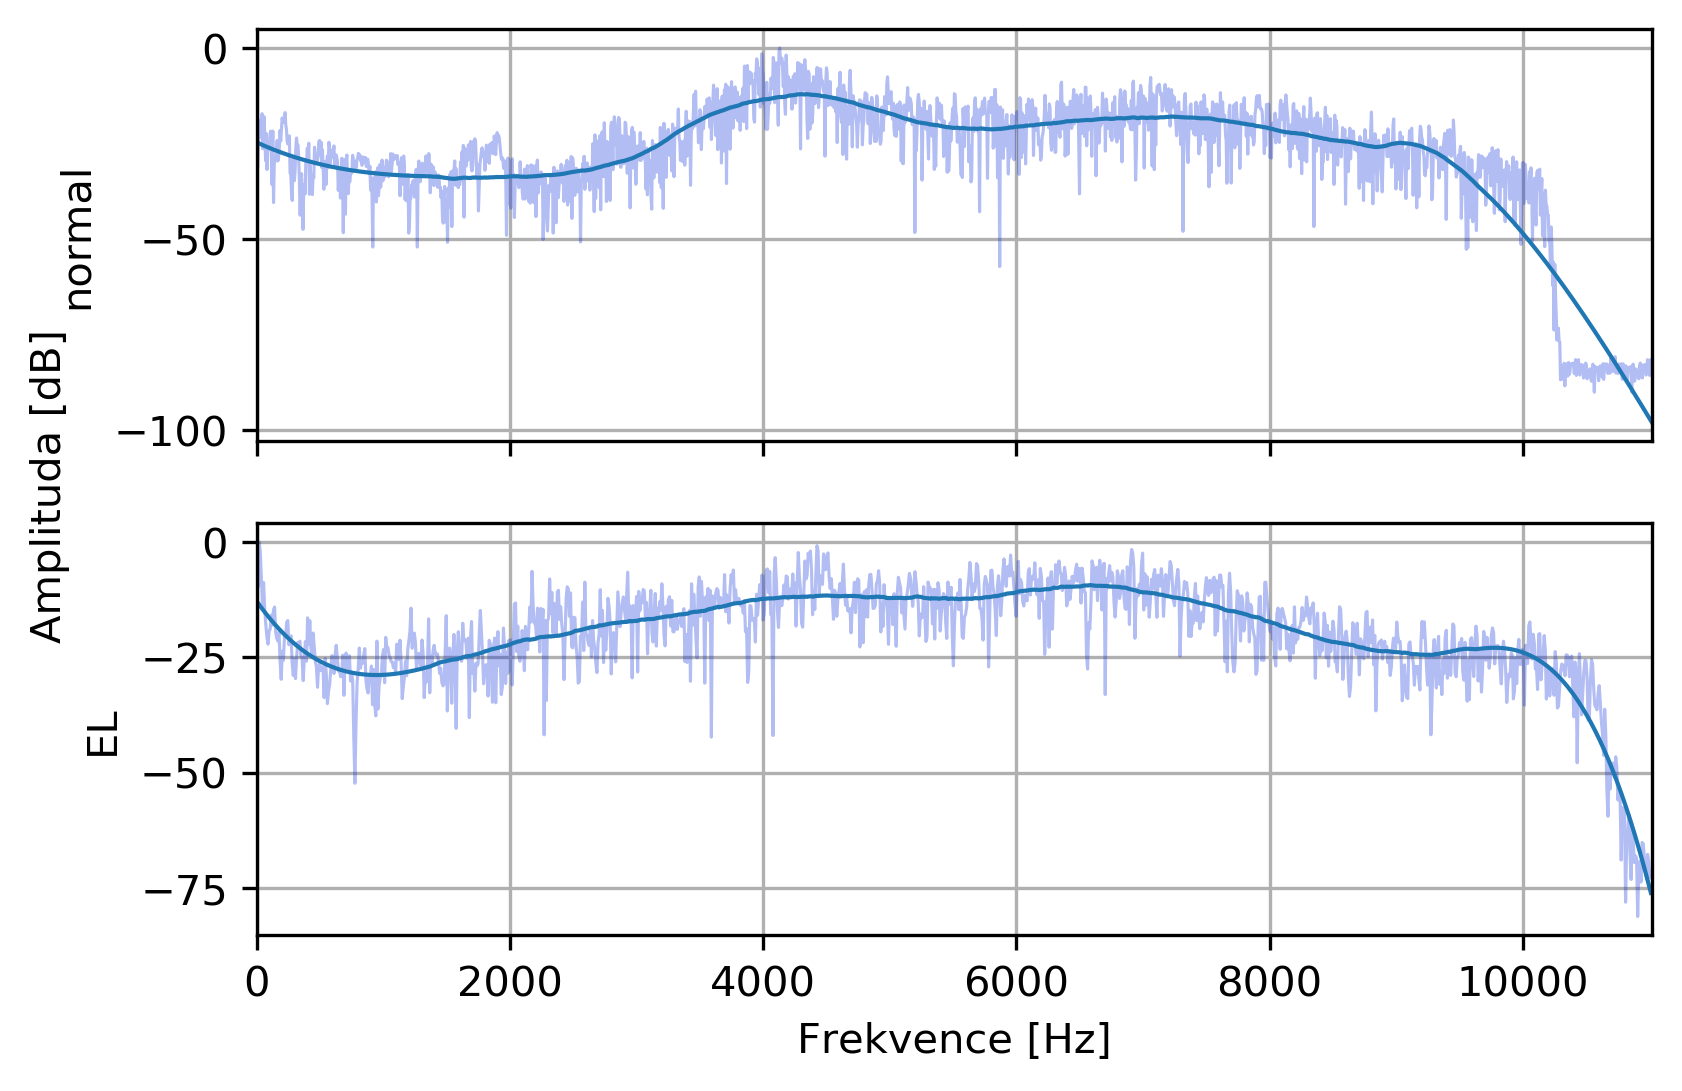
\includegraphics[width=0.9\textwidth]{./ch5-construction/img/freq_analysis_(c).png}
  \caption{Vývoj amplitudy fonému $/\check{c}/$ ve frekvenci zdravého (horní) a EL (dolní) řečníka.}
  \label{fig:construction:freq:c}
\end{figure}

Z doposud provedené analýzy plyne, že EL řeč je v mnoha charakteristikách odlišná od té produkované zdravým řečníkem. Zejména u porovnání ve frekvenční oblasti (obr. \ref{fig:construction:freq:k} a \ref{fig:construction:freq:m}) je to nejvíce patrné. Tento fakt nepochyně přispívá k tomu, že standardní obecné modely rozpoznávání řeči nedosahují takové přesnosti jako v případě bežné promluvy.

% \csvautotabular{./ch5-construction/test.csv}
